\begin{figure}[ht]
\centering
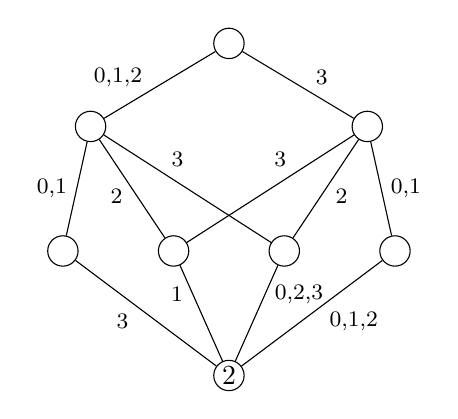
\begin{tikzpicture}[grow=down, level distance=50pt, edge from parent/.style={draw, -latex}]
    \label{fig:sea-reduced-automaton}

    \node (S) [shape=circle,draw,inner sep=1pt] {\phantom{0}};

    \node at (-50pt, -30pt) (S0) [shape=circle,draw,inner sep=1pt] {\phantom{0}};
    \node at (50pt, -30pt) (S3) [shape=circle,draw,inner sep=1pt] {\phantom{0}};
    
    \node at (-60pt, -75pt) (S00) [shape=circle,draw,inner sep=1pt] {\phantom{0}}; % 0002
    \node at (-20pt, -75pt) (S02) [shape=circle,draw,inner sep=1pt] {\phantom{0}}; % 0200
    \node at (20pt, -75pt) (S03) [shape=circle,draw,inner sep=1pt] {\phantom{0}}; % 2022
    \node at (60pt, -75pt) (S30) [shape=circle,draw,inner sep=1pt] {\phantom{0}}; % 2220

    \node at (0pt, -120pt) (F2) [shape=circle,draw,inner sep=1pt] {2};

    \path[draw] (S) -- (S0) node [midway, left, xshift=-1mm, yshift=1mm, font=\footnotesize] {0,1,2};
    \path[draw] (S) -- (S3) node [midway, right, xshift=1mm, yshift=1mm, font=\footnotesize] {3};

    \path[draw] (S0) -- (S00) node [midway, left, font=\footnotesize] {0,1};
    \path[draw] (S0) -- (S02) node [midway, left, yshift=-1mm, font=\footnotesize] {2};
    \path[draw] (S0) -- (S03) node [pos=0.3, right, xshift=1mm, yshift=1mm, font=\footnotesize] {3};
    \path[draw] (S3) -- (S30) node [midway, right, font=\footnotesize] {0,1};
    \path[draw] (S3) -- (S03) node [midway, right, yshift=-1mm, font=\footnotesize] {2};
    \path[draw] (S3) -- (S02) node [pos=0.3, left, xshift=-1mm, yshift=1mm, font=\footnotesize] {3};
    

    \path[draw] (S00) -- (F2) node [midway, left, xshift=-1mm, yshift=-1mm, font=\footnotesize] {3};
    \path[draw] (S02) -- (F2) node [pos=0.3, left, font=\footnotesize] {1};
    \path[draw] (S03) -- (F2) node [pos=0.3, right, font=\footnotesize] {0,2,3};
    \path[draw] (S30) -- (F2) node [midway, right, xshift=1mm, yshift=-1mm, font=\footnotesize] {0,1,2};

\end{tikzpicture}
\caption{SEA reduced automaton.}
\end{figure}
